\section{Passo 2 — Configurar o estudo}
\label{sec:passo2}

\subsection*{Objetivo}
Definir o contrato metodológico: o que conta como tema, o que conta como contexto, quais períodos
serão comparados, como a triagem será feita e quais estratos existirão.

\begin{figure}[H]
\centering
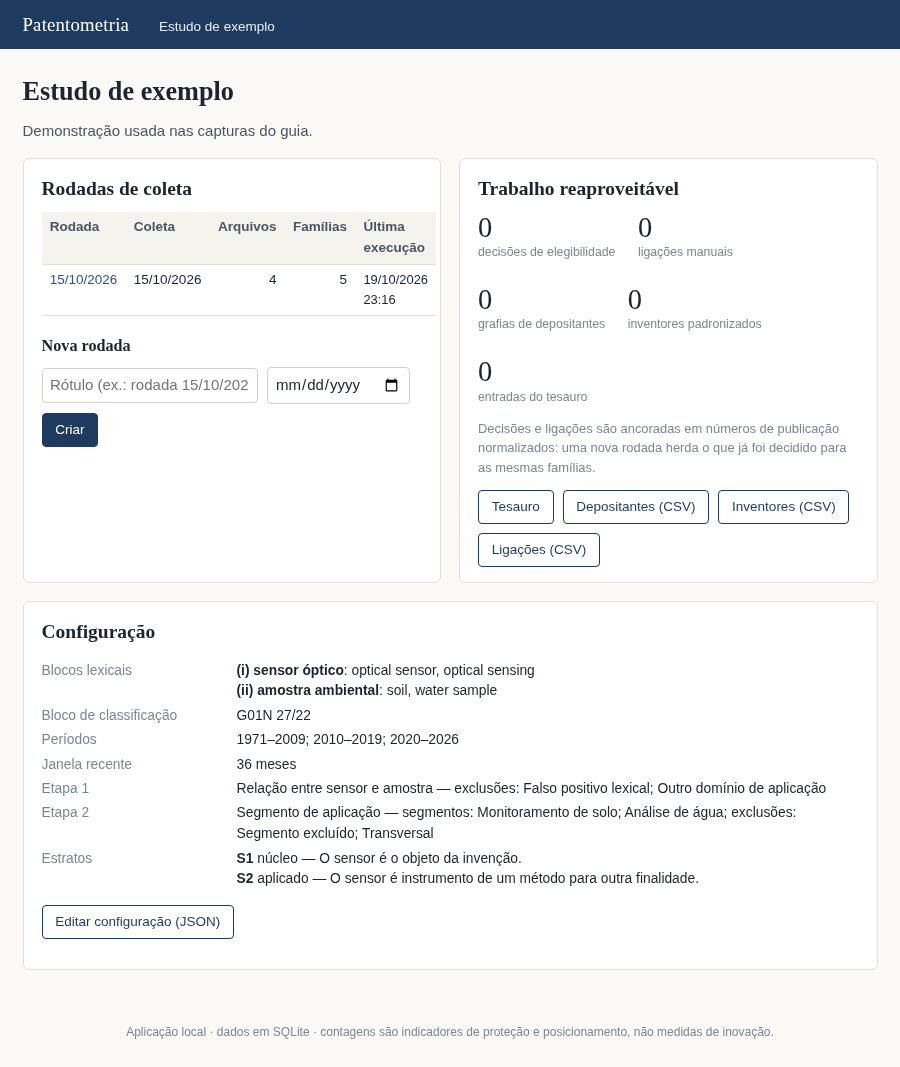
\includegraphics[width=0.72\linewidth]{img/02_estudo.png}
\caption{Painel do estudo com o resumo da configuração: blocos lexicais, classificação, períodos,
janela, categorias de triagem e estratos. O botão \emph{Editar configuração (JSON)} abre o editor.}
\label{fig:config}
\end{figure}

\subsection*{O que fazer}
\begin{enumerate}
\item Abra \textbf{Configuração} no painel do estudo.
\item Ajuste os campos do JSON (a aplicação valida antes de salvar).
\item Use \textbf{Ver tesauro} para conferir os sinônimos que serão aplicados na leitura dos títulos.
\item Clique em \textbf{Salvar} e confira o resumo que aparece no topo.
\end{enumerate}

\subsection*{Como interpretar}
Cada chave tem um efeito verificável:

\begin{itemize}
\item \campo{blocks}: grupos de termos usados para destacar o título e o resumo na triagem. O bloco
      (i) é o tema; o bloco (ii) é o contexto de aplicação. Termo genérico demais aumenta o ruído;
      termo específico demais deixa famílias fora.
\item \campo{classification\_block}: códigos de classificação usados como filtro de leitura. Não
      substituem a consulta feita na base; servem para checar aderência.
\item \campo{periods}: faixas de ano de anterioridade. Precisam ser crescentes e não se sobrepor;
      o último período é sempre parcial e deve ser lido com essa ressalva.
\item \campo{window\_months}: janela de comparação usada nos indicadores de tendência.
\item \campo{stage1}/\campo{stage2}: rótulos e motivos de exclusão. Os motivos viram categorias no
      PRISMA --- escreva poucos e mutuamente exclusivos.
\item \campo{strata}: camadas analíticas com definição textual. A definição é o que permite a outra
      pessoa repetir a classificação.
\end{itemize}

\begin{nota}[A matriz de campos]
Logo abaixo do editor, a aplicação mostra quais campos cada base exporta. Um traço não significa
zero: significa que aquela base não informa o campo. Todo indicador construído sobre um campo parcial
carrega essa lacuna, e o denominador exibido na tela é a forma de torná-la visível.
\end{nota}

\begin{alerta}[Erro comum]
Copiar a configuração de outro estudo sem revisar os blocos. Os termos de um tema não descrevem outro,
e a triagem inteira herda o erro.
\end{alerta}

\subsection*{Checkpoint}
\marcador\; O resumo no topo mostra os dois blocos, os três períodos e os dois estratos, e o botão de
validação não aponta erro.
